\documentclass[letterpaper, twocolumn]{article}
% \usepackage{usenix2019_v3}

% to be able to draw some self-contained figs
\usepackage{tikz}
\usetikzlibrary{shapes.geometric}
\usepackage{amsmath}
\usepackage{url}
\usepackage{algpseudocode}
\usepackage{algorithm}

% inlined bib file
% \usepackage{filecontents}

\AtBeginDocument{%
  \providecommand\BibTeX{{%
    Bib\TeX}}}

%-------------------------------------------------------------------------------
\begin{document}
%-------------------------------------------------------------------------------

%don't want date printed
\date{}

% make title bold and 14 pt font (Latex default is non-bold, 16 pt)
\title{3Tree: Segmented CPU Caching for Speed and Eviction Set
  Security}

%for single author (just remove % characters)
\author{
{\rm Rishav Chakravarty}\\
Dartmouth College
% copy the following lines to add more authors
% \and
% {\rm Name}\\
%Name Institution
} % end author

\maketitle

%-------------------------------------------------------------------------------
\begin{abstract}
%-------------------------------------------------------------------------------

I'll write this when I'm done with the rest of the paper as a summary of everything
\end{abstract}

%-------------------------------------------------------------------------------
\section{Introduction}
%-------------------------------------------------------------------------------

CPU caches are increasingly becoming vectors and targets for modern attacks.
The most common are software attacks that take advantage of the architecture.
Prime+Probe attacks use the sharing of a cache among multiple processes and sometimes different cores
to leak information from a different address space,
even though processes have their memory isolated from one another.
This includes attacks that use this form as their foundation,
such as speculative execution attacks
\cite{Gofetch}
\cite{Spectre}
\cite{TikTag}
\cite{PACMan}
\cite{SPAM}
\cite{LeakyWay}
\cite{Streamline}
\cite{TransientAttackSurvey}.
Rowhammer attacks use the cache to attack the DRAM modules
by repeatedly touching a memory address until the electrical interference induces a targeted bitflip
\cite{Rowhammer}.
Attacks like these are able to leak significant amounts of information from victim processes.
% How much can Spectre leak? Rowhammer? Gofetch?
Additionally, many of these attacks are difficult to detect and prevent as they occur.
Speculative attacks are especially silent,
as they work within the window of transient execution,
which completely deletes any easily accessible trace of execution after it is flushed.

Many software approaches have been introduced to defend against these attacks,
including Rowhammer-specific defenses
\cite{RowhammerDefense} % TODO: cite one more
and many defenses against Spectre and Meltdown at the OS level that are currently in use
% TODO: cite some Spectre OS defense
.

Hardware defenses are less common because changing the cache architecture can have
significant performance implications,
and preventing eviction set-based attacks completely can severely degrade
cache capacity and performance.
Instead, hardware defenses usually focus on slowing these attacks
by introducing complexity in eviction set-specific function
without overly affecting normal performance.
While software defenses benefit from being dynamic
and can be patched into operating systems and maintained applications,
many applications are archaic or unmaintained, and different hardware may secure these systems
where software alone cannot.

Both Rowhammer and Prime+Probe-based attacks use \textit{Eviction Sets}
as the foundation of their attack.
Many procedures have been introduced to very quickly discover these eviction sets,
whether for a single cache set \cite{TPFES}
or for a majority of the cache \cite{EvictionSetsAtScale}.
However, these algorithms make assumptions about the architecture,
including the use of LRU or Random replacement algorithms
and, critically, the lack of modern CPU features like 
% TODO: get examples of cache randomization from Prune+PlumTree
\cite{EvictionSetsAtScale}.
Additionally, these algorithms enable or enhance the setup for cache attacks,
but do not address the execution of the attack itself.

To this end, we introduce the \textit{3Tree} cache replacement algorithm.
The algorithm is based on software cache eviction algorithms that focus on
performance enhancement over other very commonly used algorithms,
and we implement a variation of the algorithm in hardware
with these performance characteristics in mind
and with an emphasis on security against cache priming.

% Write about the impacts of the results of this research

\section{Background}
% Introduce the concepts of caches and eviction sets

Caches are memory modules between processors and larger, slower memory modules.
They are used in many computing environments where the latency of memory
is a significant factor in performance,
such as small databases between clients and CDNs; we observe caches in CPUs.

In order to take advantage of the spatial and temporal locality characteristics
of most computing workloads,
CPU memory caches are divided into \textit{cache lines}, usually 64 bytes long,
grouped into \textit{sets} usually of 1-16 lines.
The number of lines per set is called the associativity, which we hence call $a$.
Modern CPUs use multiple levels of caches, including an L1, L2, and optional L3 cache
in order of increasing size and distance from the ALU.
The Last Level Cache (LLC) is often shared among all CPU cores, and may further group
cache sets into \textit{slices}, with one or two slices placed physically on each core.
Smaller caches tend to have lower associativity values of 2 or 4, and larger caches and LLCs
tend to have higher values between 4 and 16.

As caches are limited in size, replacement policies, also called eviction algorithms,
replace an old or stale cache line (an \textit{eviction candidate}) with a new one,
chosen based on per-object metadata.
The ideal replacement algorithm minimizes \textit{cache misses}, where the requested memory address
is not present in the cache and must wait much longer for a response
from a larger cache or main memory.
An efficient replacement algorithm will evict objects that are predicted to be unused
or will induce \textit{thrashing}, where sequential memory touches are all cache misses,
and conversely will retain objects that are commonly used
or predicted to be used again in the near future.
The miss ratio describes the efficiency of a cache:
\begin{equation}
  m = \frac{misses}{hits + misses}
\end{equation}
A cache may also be measured by its latency $T$, which describes the amount of time taken
to fulfill a memory request.
Together, the memory access time performance of a cache is given by the equation:
\begin{equation}
  T = T_{L1}(1-m_{L1}) + T_{L2}m_{L1}(1-m_{L2}) + \dots
\end{equation}

\subsection{Pseudo LRU}
% DIAGRAM: Bit Tree
% Explain how it works
% Explain what's good about it and why it's so often used
% Describe QLRU in Intel caches, why it's used, etc.

Tree Pseudo Least Recently Used (TreePLRU) is a very common replacement algorithm that
very closely follows the function of LRU.
As a perfect LRU hardware implementation requires a complex circuit and lots of energy usage,
this approximation is commonly used to approach the performance of LRU.
It organizes the cache lines into a binary tree structure to recursively divide the cache
into "hot" and a "cold" subtrees.
Each node in the tree is a single bit that 'points' to one half of the tree
(e.g. 0 points to the left, 1 points to the right).
Eviction candidates are chosen by tracing down the tree according to the direction of these nodes
following each node's colder subtree,
and address touches (including the initial placement into the cache)
trace from the node up the tree and set each node to point away from the cache line,
as the cache line should in all levels be in the "hot" subtree.
This algorithm can be easily extended into First In First Out (FIFO)
by only placing objects into the Most Recently Used (MRU) position when they are first added
and not updating the tree upon subsequent address touches.

%----------------
% TreePLRU Diagram
%----------------
\begin{figure}
\begin{center}
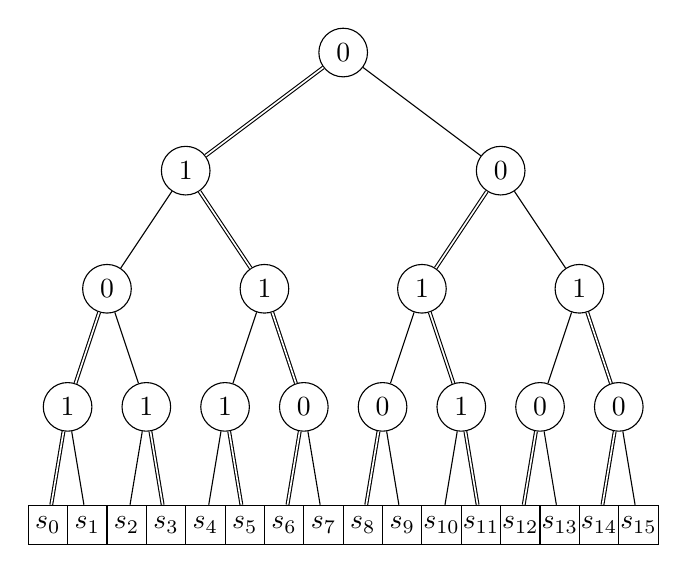
\begin{tikzpicture} [
  every node/.style={draw},
  level 0/.style={circle},
  level 1/.style={circle,sibling distance=40mm},
  level 2/.style={circle,sibling distance=20mm},
  level 3/.style={circle,sibling distance=10mm},
  level 4/.style={rectangle,minimum size=5mm,inner sep=0,sibling distance=5mm}
  ]
  \node (n0) [circle] {0}
    child {
      node (n1) {1}
      child {
        node (n3) {0}
        child {
          node (n7) {1}
          child {
            node (n15) {$s_0$}
          edge from parent [double]}
          child {
            node (n16) {$s_1$}
          }
        edge from parent [double]}
        child {
          node (n8) {1}
          child {
            node (n17) {$s_2$}
          }
          child {
            node (n18) {$s_3$}
          edge from parent [double]}
        }
      }
      child {
        node (n4) {1}
        child {
          node (n9) {1}
          child {
            node (n19) {$s_4$}
          }
          child {
            node (n20) {$s_5$}
          edge from parent [double]}
        }
        child {
          node (n10) {0}
          child {
            node (n21) {$s_6$}
          edge from parent [double]}
          child {
            node (n22) {$s_7$}
          }
        edge from parent [double]}
      edge from parent [double]}
    edge from parent [double]}
    child {
      node (n2) {0}
      child {
        node (n5) {1}
        child {
          node (n11) {0}
          child {
            node (n23) {$s_8$}
          edge from parent [double]}
          child {
            node (n24) {$s_9$}
          }
        }
        child {
          node (n12) {1}
          child {
            node (n25) {$s_{10}$}
          }
          child {
            node (n26) {$s_{11}$}
          edge from parent [double]}
        edge from parent [double]}
      edge from parent [double]}
      child {
        node (n6) {1}
        child {
          node (n13) {0}
          child {
            node (n27) {$s_{12}$}
          edge from parent [double]}
          child {
            node (n28) {$s_{13}$}
          }
        }
        child {
          node (n14) {0}
          child {
            node (n29) {$s_{14}$}
          edge from parent [double]}
          child {
            node (n30) {$s_{15}$}
          }
        edge from parent [double]}
      }
    };
\end{tikzpicture}
\end{center}
  \caption{TreePLRU metadata structure}
  \label{fig:treeplru}
\end{figure}

In Figure \ref{fig:treeplru}, 
$s_{13}$ is in the MRU position and is safest from eviction.
$s_6$ would be the first eviction candidate,
followed by $s_{11}$.

Quad Least Recently Used (QLRU) is another replacement algorithm
commonly used in Intel processors and used to replicate the function of LRU.
It is very similar to RRIP \cite{RRIP}, using four possible priority values for each cache line.
New objects are added with a low priority which gets promoted upon touches of the same address.
The object with the lowest priority is evicted, using the order of the cache lines to break ties.

\subsection{Random Replacement}
% Explain how it works
% Explain what's good about it and where it's conditionally used

Random Replacement is an eviction algorithm sometimes used in CPU caches.
Upon a cache miss, this algorithm simply chooses an eviction candidate at random.
As this algorithm does not attempt to evaluate cache lines for recency of use
or predict their next use, it suffers from a higher miss ratio than many other algorithms.
However, since it requires no cache metadata and no algorithm logic,
it uses very little energy and incurs no extra latency.
For this reason, Random Replacement is sometimes used in L1 caches,
The low latency of these caches, which is usually around 1-2ns for L1
and 4-5ns for L2 to fulfill a memory request,
means that the more common cache misses do not add too much latency to memory requests
but may save a lot of energy.
Most ARM processors equip Random Replacement algorithms in some of their CPU caches.
% TODO: cite

\subsection{TwoQ and SLRU}
% Explain how it works
% Explain what's good about it and where it's used (not hardware)

TwoQ \cite{TwoQ} and Segmented Least Recently Used (SLRU) \cite{SLRU}
are very similar eviction algorithms implemented in software,
enhancing miss ratio performance in caches for large web caches and CDNs
and for smaller-scale caches like those used in Disk-IO interaction.
They both split the LRU queue into two segments, one holding older, warmer objects
which we hence call the "hot" queue,
and one holding colder or younger objects,
which we call the "cold" queue.

Both algorithms add new objects to the cold queue
and then promote them to the head of the hot queue upon a subsequent touch.
Upon promotion, one object must be removed from the hot queue;
SLRU solves this by choosing the object in the LRU position as an eviction candidate
and placing it at the Most Recently Updated (MRU) position in the cold queue,
and TwoQ solves this by removing the object from the cache altogether.
This way, cold queue objects are isolated from the hot queue unless they are touched again,
preventing against cache thrashing and making the cache scan-resistant.

Later variations of SLRU have been introduced \cite{SSLRU},
including hardware implementations for CPU caches
\cite{DuelingSLRU}\cite{LimitedSLRU}\cite{FixedSLRU}\cite{FixedSLRUEnhancements}.
These algorithms perform well but introduce significant overhead in hardware complexity,
using bypass tables \dots

\subsection{SIEVE}

SIEVE is a simple algorithm used for large software caches as both an eviction algorithm
and as a cache primitive used as a foundation for other, more complicated algorithms.
It improves upon LRU and FIFO Reinsertion,
in which elements are placed in a FIFO queue with a \textit{safe} boolean:
upon a touch, the element is marked as safe, and upon eviction,
the first non-safe object is evicted.

SIEVE uses only one boolean of metadata per cache line, \textit{visited}
as well as a \textit{hand} to trace through the cache.
When touched, cache objects are marked as visited.
Upon eviction, the hand marches through the cache array, returning to the head if at the tail;
it evicts the first element that has its \textit{visited} bit unset,
and unsets the \textit{visited} bits of any cache objects it traces through along the way.
Instead of placing the new object at the eviction position,
the algorithm always places new objects at the head of the queue,
which prevents the new and the retained objects from being mixed together.
The hand persists its position between cache operations,
effectively resulting in a sliding window of objects at risk of eviction.

This algorithm shows significant average improvements in CDN workflow miss ratio
over many eviction algorithms,
including LRU, FIFO, ARC, and TwoQ, while being simpler than these alternatives.
It is based on principles of \textit{lazy promotion},
in which objects are only promoted at eviction time,
and \textit{quick demotion}, in which most new objects are removed quickly after their insertion.
Additionally, it significantly improves over the data usage of other
software caching algorithms, as the single boolean of metadata per line and the hand
are small and constant in memory size regardless of the capacity of the cache,
whereas timestamps for algorithms like LRU must each contain much more data,
and other index-based ordering schemes must increase their memory footprint for increasing cache size.
The algorithm also has an advantage in multithreaded software caches;
since only the visited bit of an object is set upon a cache object touch,
only cache evictions require a lock on the whole cache array.
For multithreaded applications, this vastly improves throughput,
as most other contemporary cache eviction algorithms require a whole-cache lock
both evictions and touches.

\subsection{Eviction Sets in Attacks}
% Both of the above attacks use eviction sets
% Define an eviction set very thoroughly
% Discovery and Occupation
% Actually sike covert channels can optionally use other forms
% but this is the universal way of doing it (not just Intel)
% How is it used in these attacks?

Eviction sets are an attack primitive used in many cache-based hardware attacks,
including Prime+Probe and Rowhammer.
They are used to \textit{prime} a cache by ensuring that a victim object is removed from its cache set.
An eviction set is a group of virtual addresses that are all congruent: they all map to the same cache set.
For an $a$-way associative cache, an eviction set $S$ must contain $|S| \geq a$ addresses.

The first step in eviction set-based attacks is \textit{discovery},
where an attacker must reduce a set of randmly chosen memory addresses
into a \textit{minimal eviction set}, where $|S| = a$.
Algorithms have been outlined to efficiently find eviction sets for one or almost all
of the cache sets.
% TODO: is there much else I need to write for this?

% Timing oracle
Eviction sets are used in Prime+Probe attacks as a timing oracle.
After finding eviction sets and using them to prime the cache,
an attacker times access to all items in the target cache set
before and after a victim program is run and possibly accesses elements in these target sets.
A greater time after the victim program implies that the victim accessed addresses in the victim set,
replacing eviction set elements which, upon the second access,
must introduce the significantly longer latency of a DRAM access.

Eviction sets are used in Rowhammer to bypass the cache and force DRAM hits.
By priming a cache set to evict a target congruent target address from all levels of the cache,
the target address will have to access the RAM.
Due to % TODO: what is this called
repeated RAM hits can encourage bitflips in victim memory.

\subsection{Cache-enabled Attacks}
Caches are mostly well-protected against direct attacks;
users are prevented from accessing memory placed in the cache by another process.
However, the cache can serve as a tool to enable other attacks.

\subsubsection{Transient Attacks and Forms}
Transient attacks, also called speculative execution attacks, take advantage of modern CPUs' speculative execution pipeline.
Speculative execution increases performance by guessing uncertain values that take time to evaluate, such as branch destinations
and conditions, and continuing execution under the assumption of the guess;
if the guess is later found to be incorrect, the CPU flushes the pipeline and rolls back to the last checkpoint known to be correct.

The speculative window - the period between a condition starting speculative execution and its value confirmation -
introduces a vulnerability;
If the guessed condition was incorrect, malicious code may be run in the speculative window.
Many modern CPUs, prioritizing performance, roll back only as much data as is required to continue execution
with correct functionality; code in the speculative window can leave traces in a covert channel in hardware
components where speculative misses are not rolled back.

As outlined in [source], transient execution attacks take advantage of this speculative execution window in three steps:
\begin{enumerate}
    \item \textit{Setup Phase}:
An attacker primes the microarchitectural state such that victim actions can later be decoded and intrepreted
    \item \textit{Transient Execution Phase}:
Speculative execution takes place, usually induced in a victim process by the attacker using a disclosure gadget.
The malicious code runs in the speculative window, quietly leaving a trace in the primed covert channel.
This attacking code is then squashed by the speculative execution pipeline, but the trace remains.
    \item \textit{Decoding Phase}:
An attacker decodes the information leaked into the covert channel during the Transient Execution Phase.
\end{enumerate}

As the CPU cache is too large to fully roll back upon a speculative miss, this is a common side of transient information leakage.
Previous hardware solutions to transient attacks include MuonTrap,
which introduces an additional L0-level cache that catches all speculative memory accesses
and can easily roll back upon a speculative miss.

Spectre and Meltdown, with victim-executed speculative execution and exception-induced speculative execution respectively, 
are early examples of transient attacks.
New transient attacks like PACMAN, TikTag, GoFetch, and more, use other components and features of the CPU.
These attacks follow many different forms depending on the capabilities of the hardware they run on and the
nature of the process they seek to attack.
We focus on defending against the following forms:
\begin{enumerate}
    \item \textit{Prime+Probe}:
An attacker primes a known location in cache, executes a victim program, and determines 
if the victim program accessed the primed location. This is a very common and relatively simple
type of transient execution attack.
    \item \textit{Evict+Reload}:
An attacker loads a shared binary object into its address space and primes the cache for an address
in the shared binary.
After executing the victim program, the attacker determines if the victim program accessed the primed location.
    \item \textit{Evict+Time}:
An attacker first measures the execution time of a victim program.
After priming the cache, the victim process is run and timed again.
A timing difference implies that the victim process accessed the memory affected by the cache priming.
\end{enumerate}

These attack forms are applicable to transient attacks and many others to establish a covert channel in the cache for information leakage,
and they all use eviction sets to prime the cache.
We aim to prevent or slow the use of eviction sets in the \textit{setup phase} of the transient attack, which will decrease the throughput of information leakage.

\subsubsection{Rowhammer}

\subsection{Eviction Sets}
Eviction sets are an attack primitive used in many cache-based hardware attacks.
They are used to prime a cache by ensuring that a target object is removed from its cache set.
An eviction set is a group of virtual addresses that are all congruent: they all map to the same cache set.
For a cache set with associativity $a$, an eviction set $S$ must contain $|S| \geq a$ addresses.
In a system without cache scrambling (**check on the name of this + source**), congruent addresses share index bits in their
corresponding physical address. (**check on virtual vs. physical**)

% An attacker may use an eviction set to fill a target cache set with attacker-provided objects; we refer to this process as \textit{occupation} of an eviction set.

Eviction sets are used in the following steps:

\begin{enumerate}
    \item \textit{Creation:} An attacker finds a set of congruent virtual addresses $S$ for $a$-associativity cache with $|S| \geq a$. Optionally, the attacker may choose a minimal eviction set with $|S|=a$.
    Although minimizing the eviction set can simplify the accurate detection of information leakage,
    many attacks are successful with eviction sets larger than their target caches.

    \item \textit{Occupation:} An attacker touches the memory addresses in the eviction set until the target cache is entirely filled with memory addresses from the eviction set.
    Anything previously in the cache set should be evicted through this process.
    This step is often called \textit{priming the cache} – we refer to this process as cache set \textit{occupation}.
\end{enumerate}

In rowhammer attacks, eviction sets are used to ensure that an attacker's memory request reaches DRAM.
The attacker repeatedly touches a target address, evicts the target address so subsequent accesses will not be caught by the cache,
and re-references the target address.

In transient attacks, a target address is usually evicted as part of a timing attack, as a memory request to an evicted object
must take time to travel to and from DRAM, and this timing difference is significant enough to be measured
by high-performance counters or simply by a continuously incrementing variable.
In Prime+Probe, the attacker occupies the cache set of a target address, executes the victim program, and re-references
all the addresses in the eviction set; an increase in the time taken implies that the target address was referenced and evicted
one of the objects of the eviction set.
In Evict+Reload and Evict+Time, the attacker measures the victim's runtime before and after occupying a cache set,
with a longer re-run time implying a reference of an evicted cache object.

We primarily aim to slow cache set \textit{occupation}.
Most eviction set attacks create eviction sets once but use them for occupation many times;
by slowing occupation, we reduce the information leakage throughput of these attacks
and possibly reduce the likelihood of rowhammer bitflips.

\section{Design}

We seek to make rowhammer-style and transient execution attacks more difficult by preventing or slowing the use of eviction sets
using hardware-level cache eviction algorithms.
Additionally, we aim to accomplish this security without inducing a significant performance hit in the cache of either miss rate or latency.

\subsection{Expected Difficulty of an Eviction Algorithm}
We define the difficulty of occupying a cache set with a certain touching pattern as the total number of memory touches
required to overwrite all lines in the cache with addresses from an eviction set.
With this measurement, we evaluate the LRU (and its variants) and Random Replacement eviction algorithms for their security against cache set occupation.
We use these measurements as baselines of comparisons for our own cache eviction algorithm.

For the minimum difficulty, we assume an optimal attacker;
for each eviction algorithm, there exists a memory touching pattern that most effectively fills a cache set.
We define the minimum difficulty of an eviction algorithm as the number of optimally-ordered touches required to fill a cache set.

Additionally, randomness is a factor in some of these eviction algorithms.
We assume a uniform random distribution of initial cache states;
for some algorithms, the initial state into which an attacker would start placing eviction set objects affects the order of evictions.
Additionally, some algorithms use randomness in selecting an eviction candidate.
We define the expected minimum difficulty of an eviction algorithm as the mean number of optimally-ordered touches required to fill a cache set.

\subsubsection{LRU, TreePLRU, and FIFO}
% Derive expected difficulty, no choice or permutation randomness
LRU, TreePLRU, and FIFO pose little defense against cache priming.
In both FIFO and LRU caches, new cache objects are instantly promoted to the head of the queue.
In LRU, new objects are marked as the most recently updated and thus the last to be evicted,
and the FIFO queue means new objects are evicted after objects added earlier.
Although TreePLRU does not follow the same linear structure,
it is similarly trivial to occupy a cache set.
Thus, for an $a$-way associativity LRU, FIFO, or TreePLRU cache, an attacker only needs
$a$ sequential touches to fill a cache set.
As these algorithms are deterministic, the expected difficulty is the same value.

\begin{equation}\label{LRUExpectedD}
  D_g(LRU) = D_{m}(LRU) = D_{Em}(LRU) = a
\end{equation}

\subsubsection{Random Replacement}
Given a cache set with associativity $a$ in which an attacker has occupied $n$ addresses
using some subset $S \subset E, |S| = n$ of eviction set $E$,
a following touch on address $\alpha$ may be in $S$ or not.

If $\alpha \in S$, there is no cache or per-line metadata to update, and the cache state does not change.

If $\alpha \notin S$, the random replacement algorithm will evict an address $\beta$.
This evicted address will occupy an unoccupied line with probability
$P(\beta \notin S) = \frac{a-n}{a}$.

Then, the probability occupying $n+1$ addresses in a cache set with $n$ addresses occupied is $P(n+1) = \frac{a-n}{a}$.
The corresponding expected value is $EV(n+1) = \frac{1}{P(n+1)} = \frac{a}{a-n}$
Then, the expected value of the total number of unique touches to occupy an eviction set is

% If they have an issue with this not being fully simplified they can take that up in review
\begin{equation}\label{RandomExpected}
    D_g(Random) = D_{Em}(Random) = \sum_{i=0}^{a-1}{\frac{a}{a-i}}
\end{equation}

\subsection{Preventing Eviction Set Occupation}
Attackers use eviction sets as attack primitives to guarantee that a target address is not present in the cache
so a victim's memory request of the target address must travel to DRAM and back.
Leaving at least one of the lines in a cache set open and unoccupied means that attackers have no guarantee that the target address is evicted.
Thus, to slow the use of an eviction set in occupying a cache set, we must only increase the difficulty of the eviction algorithm used.

\subsection{Latency and Energy Costs}

As the CPU implements eviction algorithms in hardware, the function of some software-based algorithms
may not be exactly reflected without inducing significant performance or complexity overhead.
For example, LRU can be implemented in a software cache to add, update, and remove objects in $O(1)$ time.
Although no such time complexity exists for algorithm circuitry that runs in parallel,
exact LRU is complex in CPU caches and involves lots of metadata per cache line and lots of circuitry to
determine an eviction candidate.
Excessive circuitry introduces extra latency by increasing the critical path of the circuit
and extra energy usage by requiring additional transistors.
The LRU algorithm is thus commonly simplified to TreePLRU in the CPU, which requires much less hardware complexity
but achieves a similar miss ratio.
Although the energy usage can be significant, modern CPU features like prefetching largely mitigate the latency factor of the algorithm.
Additionally, many modern CPUs punt the cache eviction calculation to after fulfilling the memory request.

Additionally, the cache - other than random replacement caches - may introduce registers for the cache metadata used in eviction.
However, the amount of metadata is much smaller than the amount of data in a cache set:
for an 8-way associative, 64-byte cache line, a TreePLRU replacement policy for the set uses
$\frac{7}{512 \cdot 8}=0.17\%$ as much space as the data itself.
Thus, within reason, we treat metadata usage as insignificant compared to the space and energy usage of the cache.

For the sake of simplicity and due to the lack of comparison against proprietary CPU cache implementations,
we analyze and evaluate our eviction algorithm qualitatively.
% I mean to say that we only check that the value is reasonable and move on,
% because that's all I can do

\subsection{Miss Rate Cost}

\section{Implementation}

As discussed in 3.3, due to the hardware requirements and parallel nature of circuits,
we implement our cache eviction algorithms as approximations of their software equivalents.
We implement and discuss multiple variants of each algorithm.

\subsection{SIEVE}

SIEVE, as implemented in software, does not translate well to hardware.
It relies on entirely sequential logic to determine an eviction candidate;
additionally, it conditionally returns the hand to the beginning of the cache array.
These two features imply the use of a register to keep track of the hand position,
constant updating to reflect its marching through the cache array
and its possibility of returning to the beginning of the array.
Along with an increased hardware footprint, this would result in immense energy usage,
especially compared to other algorithms like TreePLRU that select an eviction candidate
without sequential logic at all.

\subsection{2Tree}

TwoQ does not rely on sequential logic nearly as much as SIEVE,
but there are multiple possible ways to implement the dual-queue structure.
I implement TwoQ as a tree structure very similar to TreePLRU.
The cache is split into two smaller queues, each with their own subtree:
the \textit{cold} queue, containing $\frac{1}{4}$ of the elements,
and the \textit{hot} queue, containing $\frac{3}{4}$ of the elements.
The hot queue, having a multiple of 3 elements,
is further split into
a \textit{probation} segment, containing $\frac{1}{4}$ of the total elements,
and a \textit{safe} segment, containing the remaining $\frac{1}{2}$ of the elements.
We choose a tree-based replacement policy for each of the two subtrees,
and additionally define a \textit{choice} probability $c$.

With this structure, the cold tree,
not including the cache lines themselves as leaf nodes, has height $log(a) - 2$.
Thus, this algorithm is not possible for caches with $a < 4$.
We implement and test this algorithm only for 4-, 8-, and 16-way associativity.

New elements are added to the cold queue with probability $1 - c$
or to the probation segment of the hot queue with probability $c$.
If added to the cold queue, an eviction candidate is selected from the cold queue
according to the cold queue's replacement algorithm;
if added to the probation queue, the eviction candidate is selected using the replacement algorithm
of the hot queue, but limited to the subtree of the probation queue.
When an object $a$ in the cold queue is touched again
or a new object is added directly to the probation queue,
an eviction candidate $b$ is chosen from the hot queue according to its replacement algorithm.
The entire cache line of $a$ is swapped with that of $b$,
and $a$, now in the hot queue, is promoted according to the hot queue's replacement policy.
$b$, now in the cold queue, is not promoted.

\begin{algorithmic}
  \State $i \gets 10$
\end{algorithmic}

\subsection{3Tree}

We implement 3Tree with three tree structures similar to 2Tree and TreePLRU.
The cache is split into three separate subtrees:
\begin{itemize}
\item the \textit{cold} queue, containing $\frac{1}{4}$ of the elements
\item the \textit{probation} queue, containing $\frac{1}{4}$ of the elements
\item the \textit{hot} queue, containing $\frac{1}{2}$ of the elements.
\end{itemize}
Like 2Tree, we choose replacement algorithms for each of the three subtrees,
and define choice probabilities $c_{cold}$, $c_{prob}$, and $c_{hot}$ as parameters,
with $c_{cold} + c_{prob} + c_{hot} = 1$.
Like 2Tree, the smaller trees prevent use of the algorithm for $a < 4$.

When adding a new element $a$, one of the subtrees is chosen according to their choice probabilities.
We choose $c_{cold} = \frac{1}{2}$, $c_{prob} = \frac{3}{8}$ and $c_{hot} = \frac{1}{8}$
for all implementations and testing.
Then, an eviction candidate $b$ is selected from this subtree according to its replacement policy
and a 

\section{Experiment Methodology}

% Eviction set functions
To evaluate 3Tree in comparison to other algorithms in their defense
against eviction set-based cache priming, % TODO: maybe change this to "eviction set function"
we implement a cache simulator to represent an attacker.

% Performance
To evaluate the performance of 3Tree, we implement the algorithm in the
cycle-accurate gem5 CPU simulator on the SPEC2017 suite of benchmarks
to reflect common computing workloads.
Some of these workloads depend on the memory subsystem more than others,
but we take the benchmark suite as generally representative
of cache workloads.

\section{Results}

\section{Discussion}

% PARSEC
% SPEC, if I can get it working
% Custom/synthetic workloads

%-------------------------------------------------------------------------------
\bibliographystyle{acm}
\bibliography{sources}

%%%%%%%%%%%%%%%%%%%%%%%%%%%%%%%%%%%%%%%%%%%%%%%%%%%%%%%%%%%%%%%%%%%%%%%%%%%%%%%%
\end{document}
%%%%%%%%%%%%%%%%%%%%%%%%%%%%%%%%%%%%%%%%%%%%%%%%%%%%%%%%%%%%%%%%%%%%%%%%%%%%%%%%

%%  LocalWords:  endnotes includegraphics fread ptr nobj noindent
%%  LocalWords:  pdflatex acks
